%% Introduction 
%%	What is this chapter all about? 
%%	What sub-problem or issue is this chapter addressing? 
%%	How does this chapter fit within the overall “story” of the thesis? 
%%The Meat
%%	Rigorous approach to sub-problem, or detailed explanation of issue
%%	Assumptions underlying sub-problem, or complete description of issue
%%	Validation: System design, theory, implementation, graphs, references, …. 
%%Summary
%%	Repeat the highlights of the chapter
%%	Transition sentence that acts as a “teaser” for the next chapter, and how the next chapter fits with the current one
	

\section{Introduction}

This chapter presents \replaced{an approach}{process} for feature generalization where sheet metal feature based CAD model is transformed into generalized feature based CAD model. It begins by establishing the need for generalized features and then presents the methodology for building generalized feature based CAD model based on Spatial Grammar technique. \deleted{The proposed model is called as $\mathcal{ABLE}$. Later, transformation of sheet metal feature based CAD model to $\mathcal{ABLE}$ model, is elaborated.} Towards the end, this chapter demonstrates the ease with which midsurface computation can be performed on such CAD model.
\todo{Review comment: First bring out the need of generalized feature representation in the context of midsurface generation. This should be high level. [ADDED THE NEXT PARA]}
\deleted{The present research attempts to use Loft as a generalized feature form to represent CAD features in the sheet metal domain.}
Following section details out the need for generalized feature based CAD model representation.

\section{Need for Generalized Feature Representation}

Feature based CAD models are widely used in development of products from different domains, such as plastics, machining, sheet metal, etc. These domains have their own feature types as per the vocabulary of the domain. For example, sheet metal domain has its own set of features such as Flange, Bend, Slots, Rip, Hem, etc. 

%%\bigskip

	\begin{figure}[!h]
	\centering
	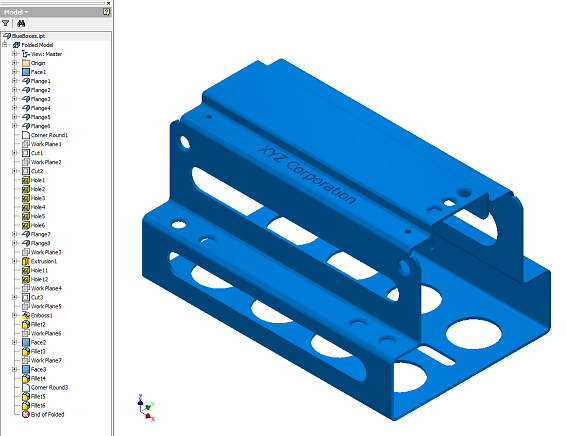
\includegraphics[width=\linewidth]{images/blueboxes}
	\caption{Sheet Metal CAD Model and Feature Tree}
	\label{fig_ariplainpair}
	\end{figure}

	\begin{figure}[!h]
	\centering
	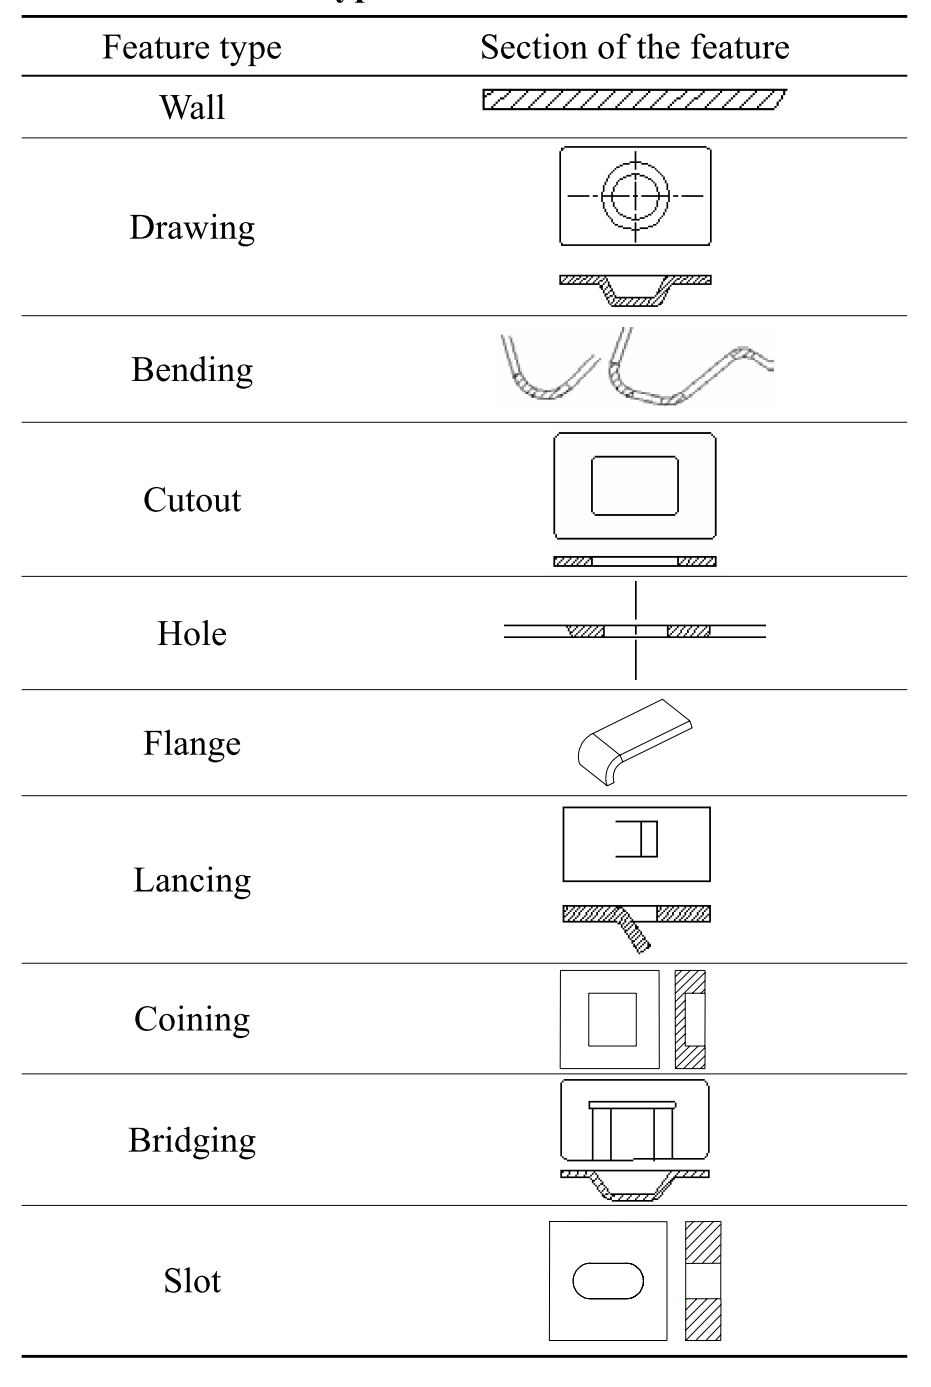
\includegraphics[width=0.5\linewidth]{images/liuFeatures}
	\caption{Sheet Metal Features}
	\label{fig_smtaxonomy}
	\end{figure}
%%
%%\begin{figure}[h!]
%%\centering     %%% not \center
%%\subfloat[Sheet Metal CAD Model and Feature Tree]{\label{fig_ariplainpair}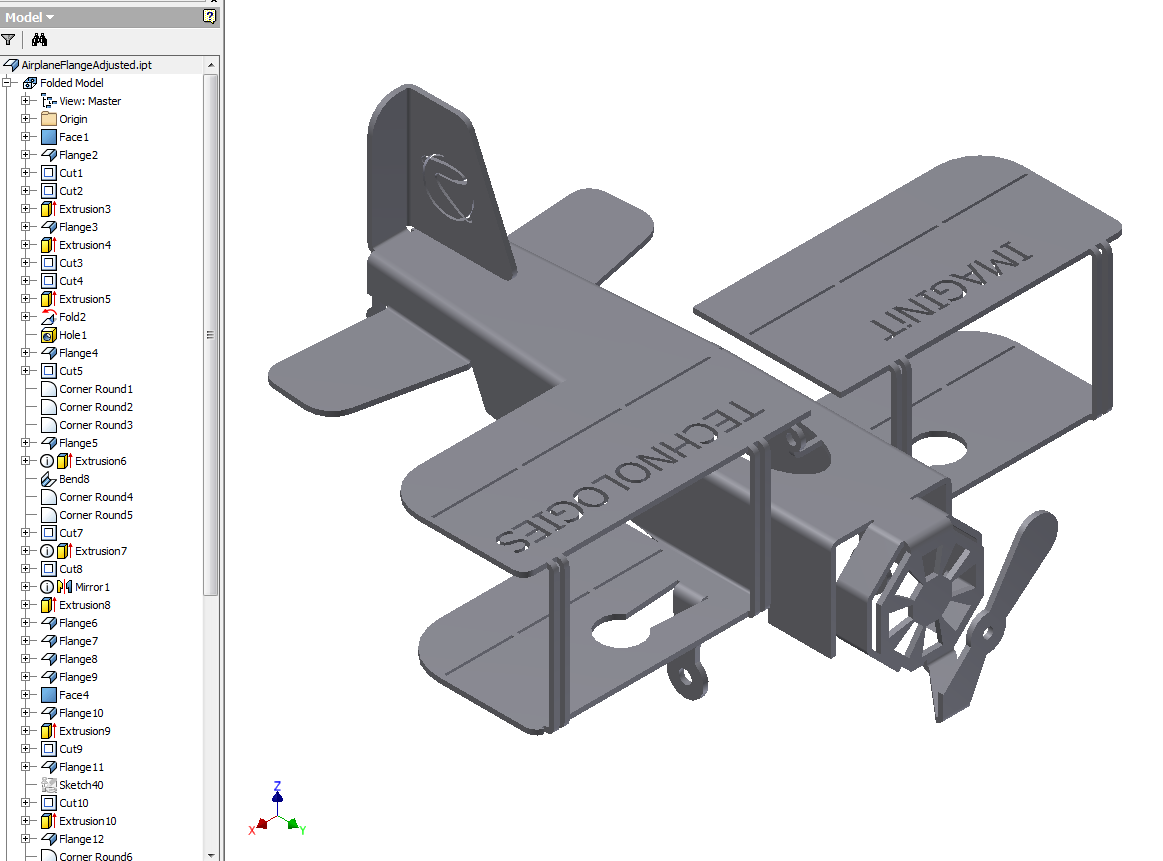
\includegraphics[width=0.63\linewidth]{images/airplanefeatures}} \hfill
%%\subfloat[Sheet Metal Features]{\label{fig_smtaxonomy}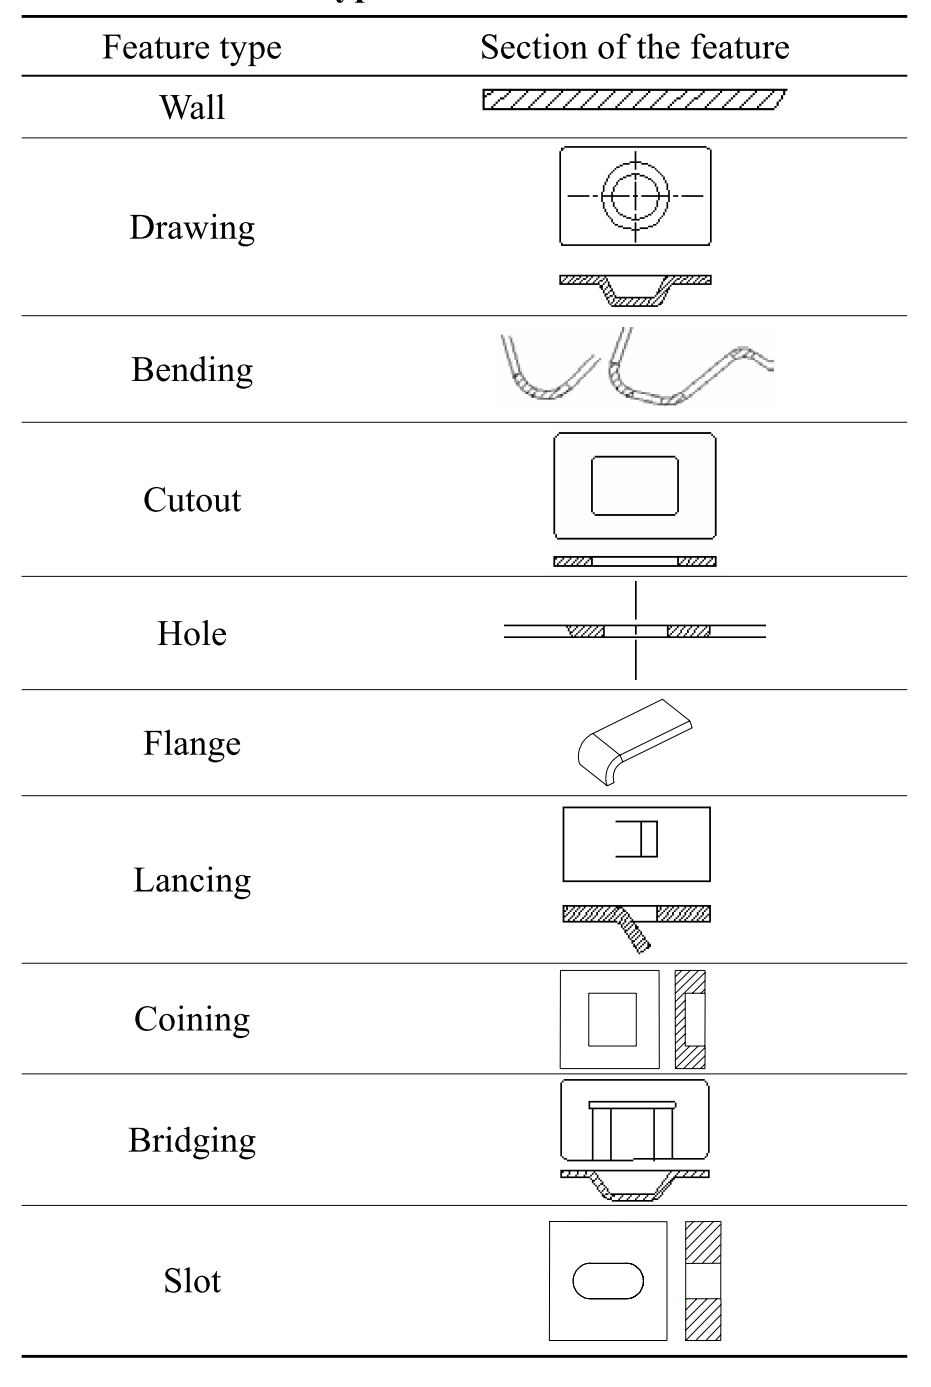
\includegraphics[width=0.32\linewidth]{images/liuFeatures}} 
%%\caption{Variety of Sheet Metal Features}
%%  \label{fig:able:variety}
%%\end{figure}

%%\bigskip

\todo{Review comment: Show with an example how too much variety of features can make midsurface generation a complex problem and vis a vis how same model with very generalized primitive features can ease out midsurface generation. [DONE. ADDED EXAMPLE AND Figure \ref{fig_ariplainpair}]}
Figure \ref{fig_ariplainpair} shows a typical sheet metal part along with various features used in its construction such as Face, Flange, Bend, Cutout, etc. Figure \ref{fig_smtaxonomy} shows widely used sheet metal feature types. Actual number of feature types could be in the range of 60-70 for sheet metal domain only~\cite{Inventor2014Help}. Although such diversity of features gives immense flexibility, power to the designers \added{\& modelers} to build desired models, but it can be challenging for downstream applications. So, the existing feature-based midsurface computation approaches need to develop separate computation logic for each of these features~\cite{Robinson2006, Stolt2008, Cao2009}. Large number of feature types thus require huge effort in the design and implementation of midsurface computation algorithm. To avoid this problem, a solution has been proposed in the present research work. It has devised a generic feature form by \replaced{the concept}{process} of generalization. All CAD features are transformed into a smaller set of generalized features, making it easier to write \replaced{the midsurface computation algorithm}{a feature-based algorithm}. 

\todo{Review comment: Why jump to hypothesis 6 without any intro/context. [REMOVED]}
\todo{Review comment: Then mention that ...simplifying the CAD model in terms of generic feature tree that can reduce the complexity of midsurface computation to a great extent. [MENTIONED HERE]}
\todo{Review comment:  Whether this need has been felt earlier by researchers and what was their problem and how they solved it. Introduce Spacial grammar concept here. [DONE]}

\added{The problem of a wide variety of features has been encountered in the past as well. Some researchers used cellular decomposed model to address this for computing midsurface ~\cite{Cao2009}. The CAD model was decomposed into solid cells. The cells were subjected to feature recognition into standardized features such as Extrude~\cite{Boussuge2013a}. Then the midsurface was computed for the Extrudes. Although these approaches work for simple models, they fail on the real-life models due to inability to recognize standard features on decomposed cells. Shapes of cells may not conform to the chosen standardized feature such as Extrude. Another problem was that, during decomposition, the original design intent would get lost which is not recovered by the feature recognition. Thus these approaches have not worked effectively in computing midsurface. The present research addresses these issues as elaborated in the following sections.}

\added{Although the reduction in variety of features helps in reducing the cases to be dealt while writing midsurface algorithm, it would further help if these small set of features themselves be represented by generalized transformations on basic geometric entities. Spatial Grammar~\cite{Stiny1971}, which is widely used in generative design and architecture, etc., describes construction of shapes using transformations of simple geometric entities. These entities and transformations on them are tersely represented by notations known as Spatial Grammar.}
%%In the same context, it proposes and tests hypothesis \ref{hyp:Abstraction}.
%%
%%\begin{myhyp} \label{hyp:abstraction:loft}
%%CAD features can be represented as a single or combination of Loft features  having multiple profiles and a guide curve.
%%\end{myhyp}

%%Lofting, with inputs as $sketches$ and a $guide curve$, is a versatile generic operation. Different geometric shapes can be built by lofting different $sketches$ along with the different $guide curve$s. Table ~\ref{tbl:abstraction:entitiesfeaturesusingable} shows how various entities could be represented using just a $sketch/profile$ and a $guide$. With $Point$ as a fundamental entity, other geometries can be defined by formulating the $sketch$ which is swept along the $guide curve$. 
%%
%%\begin{table}[!htb]
%%\begin{tabular}[h]{@{}p{0.25\linewidth} p{0.18\linewidth} p{0.18\linewidth} p{0.18\linewidth}@{}}
%%\toprule
%%%\backslashbox[1mm]{sketch}{guide} & {\bf line} & {\bf arc} & {\bf curve}\\
%% $sketch\downarrow , guide\rightarrow$   & {\bf line} & {\bf arc} & {\bf curve}\\
%%\midrule
%%{\bf point} & line & arc & curve \\\midrule
%%{\bf line} & plane surf & cylinder surf & ruled surf\\\midrule
%%{\bf arc} & cylinder surf & torus surf & saddle surf \\\midrule
%%{\bf open profile} & ruled surf & circular surf &  free form surf \\\midrule
%%{\bf rectangle} & box & rect torus & rect sweep \\\midrule
%%{\bf circle} & cylinder (surf/solid) & torus (surf/solid)  & tube (surf/solid) \\\midrule
%%{\bf closed profile} & Extrude  (surf/solid) & Revolve (surf/solid) & Sweep (surf/solid) \\\midrule
%%%\bottomrule
%%\end{tabular}
%%\caption{Sweeping based Entities}
%%\label{tbl:abstraction:entitiesfeaturesusingable}
%%\end{table}
%%
%%For example, with $rectangle$ as a $sketch$ and a $line$ as a $guide$ results in a solid $box$ (``Solid'' output option is assumed here. In case of ``surface'' as an output option, open surface box will be created).
%%
%%
%%As the present research focuses on sheet metal parts and one of the peculiarities of them is that they are typically constant thickness models. In this case, Sweep, rather than Loft, is the most appropriate generic form of abstraction. A sweep is a special case of Loft where, instead of multiple profiles, a single profile and a guide curve is specified. Extrude and Revolve are special cases of Sweep, so are used interchangeably to be equivalent forms.

The present research uses Spatial Grammar notations to represent the generalized feature form and has been detailed below. \deleted{Spatial Grammar can be effectively used to represent the neutral form feature representation.}

\section{Related Research}

Following subsections report literature on some of the domains relevant to feature generalization, such as Spatial Grammar and Feature Representation.
% (Definition  \ref{def:formfeature}) representation.  
%
%\begin{mydef}
%\label{def:formfeature}
%Form feature is a local shape (geometric and topological) that has engineering significance.
%\end{mydef}

\subsection{Spatial Grammar Approaches}

\todo{Review comment: Introduce this in earlier section. (or) Drop this [NOT CHANGED AS THE INTRODUCTION LOOKS APPROPRIATE HERE]}

Spatial Grammar is a general term which encompasses various shape definition grammar, like Graph Grammar, Set Grammar etc.~\cite{mckay2012}. Aim of Spatial Grammar is to bring formalism through terse but expressive definitions, validations and generation of new evolutionary shapes. 

Spatial Grammar\deleted{in a generative approach} was formally introduced by Stiny and Gips~\cite{Stiny1971} and is primarily used for exploratory, evolutionary design process. It is defined by set of shapes, labels and rules for geometric transformations. An example rule, say $A \rightarrow B$ first finds a shape with label $A$ and then applies the geometric transformation suggested by the rule and outputs the result $B$. 

\todo{Review Comment; Elaborate further. Don't give any conceptual understanding. [ADDED FIGURE AND FEW LINES EXPLANATION]}

%%\bigskip

	\begin{figure}[!h]
	\centering
	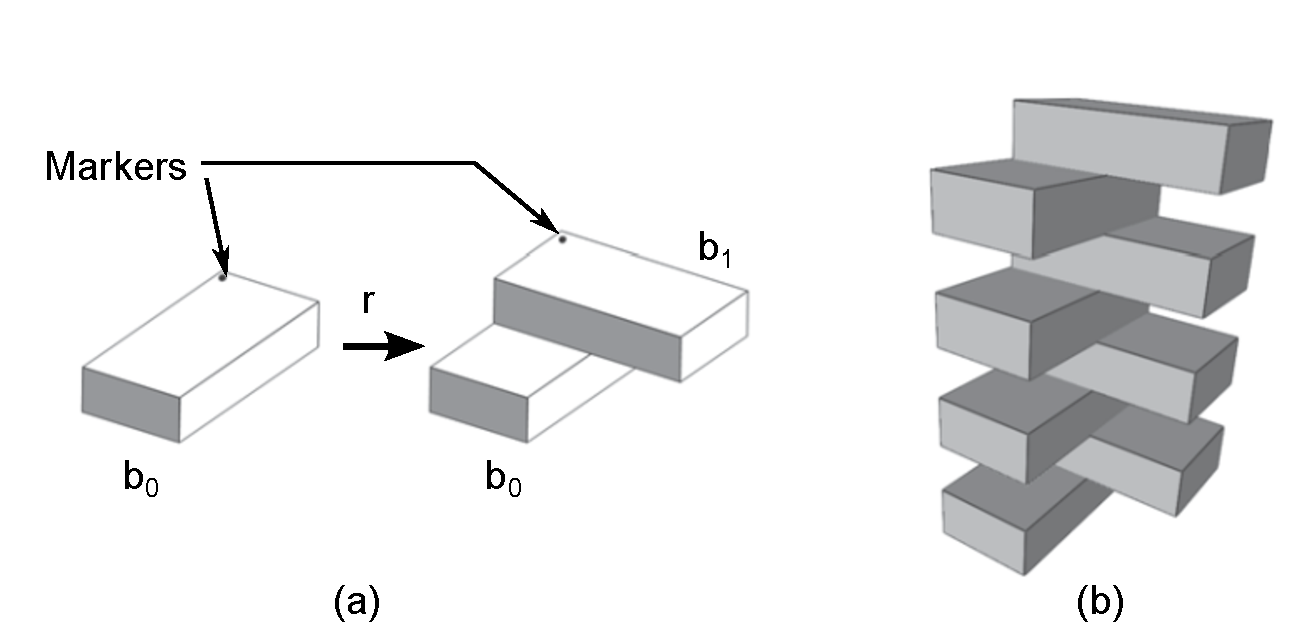
\includegraphics[width=0.62\linewidth]{images/stinyrules.pdf}
	\caption{Shape Grammar Rule (Source: Hoisl~\cite{Hoisl2009})}
	\label{fig:able:StinyRules}
	\end{figure}


%%\bigskip

	
Figure \ref{fig:able:StinyRules}(1) shows a sample rule, say, $r$, where a newer block ($b_1$) is placed on the earlier block  ($b_0$) orthogonally, after matching the marker dots. This rule, when applied successively $n=7$ times, results in the shape shown in Figure \ref{fig:able:StinyRules}(2). The resultant model can be represented by $n \times r(b)$. Thus a shape can be represented by an expressive and terse notation. Using variety of such rules, it is possible to build shapes. Inspite of these advantages its usage in the mainstream design applications appears marred due to complexity of defining and editing the rules.

Hoisl et al.~\cite{Hoisl2009} proposed a Spatial Grammar based system, with implementation in CAD\deleted{for generative solutions}. They used primitives like block, cylinder, cone as initial shapes and proposed use of \replaced{Sweep feature}{{\em sweeping}} to generate different shapes depending on different profiles and guide curves. Boolean operations were used to build more complex shapes. 

CAD Grammar proposed by \added{Deak}~\cite{Deak2006} combined Shape and Graph Grammar to be more useful in Design, Modeling and Manufacturing. He claimed that traditional Shape Grammar could not work well with the CAD primitives\deleted{ and it would be desirable to have such a representation that will work with different CAD systems}.

\added{Moustapha~\cite{Akin2004, Moustapha2004, Hoda2005} developed interactive geometric configuration system based on Shape Grammar for architectural designs. Transformation rules were similar to language grammar rules. Although, with a wide variety of transformations, it was possible to generate different shapes, it lacked one of the key property, i.e. uniqueness. There is no process for recognizing spatially equivalent, yet, notationally different configurations. }

Apart from Spatial Grammar related approaches there have been attempts to devise generalized (also known as `neutral') feature form with which CAD models are built. This is elaborated briefly in the following subsection. %Following subsection elaborates those in brief.

\todo{Review Comment: Survey table not needed. [REMOVED]}

%
%\csvreader[longtable=|p{0.15\linewidth}|p{0.15\linewidth}|p{0.15\linewidth}|p{0.2\linewidth}|p{0.17\linewidth}|p{0.17\linewidth}|,
%    table head=\toprule \bfseries Author & \bfseries Input& \bfseries  Method & \bfseries  Approach& \bfseries  Advantages& \bfseries  Limitations \\ \midrule \endhead,% \bottomrule \endfoot,
%  late after last line=\\\bottomrule,
%  before reading={\catcode`\#=12},after reading={\catcode`\#=6},    
%    late after line=\\\hline]%
%{litsurvey_grammar.csv}{Author=\Author, Input=\Input, Method=\Method, Approach=\Approach, Advantages=\Advantages ,Limitations=\Limitations}%
%{\Author  & \Input&  \Method &\Approach & \Advantages & \Limitations}%


\subsection{Feature Representation Approaches}

A feature-based CAD model is built using features. Each feature adds, modifies, deletes a solid volume, thereby transforming the existing model. So, feature is a similar entity in building a CAD model, as a rule in the Spatial Grammar. Features are specific to applications, such as sheet metal, manufacturing, etc. Due to a large variety of features, developing a generic feature-based algorithm is cumbersome. Many researchers have attempted to either devise a generalized feature form or present feature class hierarchy (taxonomy) so that similar features can be treated similarly in the algorithm. \deleted{A generally accepted definition of a feature is that  it represents shape as well as functionality significant to a particular product life-cycle phase~\cite{Berg2002}.  Features embed application specific high level knowledge and manifest differently as per the context~\cite{mandorli1996}.}


%%\bigskip

	\begin{figure}[!h]
	\centering
	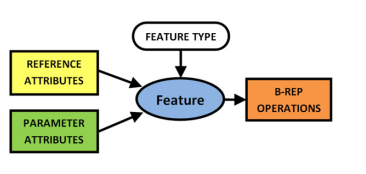
\includegraphics[width=0.5\linewidth]{images/OntologyTessier}
	\caption{Feature Ontology (Source: Tessier~\cite{Tessier2013})}
	\label{fig:litsurvey:Tessier}
	\end{figure}


%%\bigskip

\deleted{Features through use of taxonomy, semantics and ontology  bring formalized knowledge representation which can be leveraged to address problems such as interoperability between CAD system and developing downstream applications such as CAE, CAM etc~\cite{BidarraBronsvoort2000},~\cite{Tessier2011},~\cite{Ma2013}. }
	  
In figure \ref{fig:litsurvey:Tessier} Tessier showed that the generalized feature form can be represented using feature-type, solid body (B-rep) geometry and attributes. 
	  
Middleditch~\cite{Middleditch1997} provided abstract definition for geometric features based on cellular structure, which supported design, manufacturing applications. 

Brunetti~\cite{Brunetti2005} combined parametric modeling with ontological reasoning for application of feature interoperability. His semantic-based shape representations was applicable to different engineering tasks using application specific ontologies.	  

\todo{Review Comment: Survey table and Observations not needed. Instead of these observations have a separate paragraph or a section to explain how shape grammar concept can be leveraged for midsurface problem. How and why it has a potential for the same. has anybody used shape grammar this way? If not say that you have proposed an approach for this. [REMOVED AND ADDED A PARA BELOW]}

%%
%%	
%%\csvreader[longtable=|p{0.15\linewidth}|p{0.15\linewidth}|p{0.15\linewidth}|p{0.2\linewidth}|p{0.17\linewidth}|p{0.17\linewidth}|,
%%    table head=\toprule \bfseries Author & \bfseries Input& \bfseries  Method & \bfseries  Approach& \bfseries  Advantages& \bfseries  Limitations \\ \midrule \endhead,% \bottomrule \endfoot,
%%  late after last line=\\\bottomrule,
%%  before reading={\catcode`\#=12},after reading={\catcode`\#=6},    
%%    late after line=\\\hline]%
%%{litsurvey_featureontology.csv}{Author=\Author, Input=\Input, Method=\Method, Approach=\Approach, Advantages=\Advantages ,Limitations=\Limitations}%
%%{\Author  & \Input&  \Method &\Approach & \Advantages & \Limitations}%

%%\subsection{Observations from Related Approaches}
%%
%%%
%%\begin{itemize}[noitemsep,topsep=2pt,parsep=2pt,partopsep=2pt]
%%	\item In general there has been limited success to the usage of Spatial Grammar in CAD and in the downstream applications, so far, especially for the purpose of neutral {\em feature} definitions.
%%	\item  As this work focuses on thin-walled solids, so naturally scopes itself to work on Sheet Metal features. Use of Spatial Grammar notations to represent scheme of generalized {\em form features} is relatively new and is not widely utilized in the commercial CAD applications. 
%%	\item This work formalizes an approach to  the neutral form-feature representation and later uses it to develop the midsurface computation algorithm.
%%\end{itemize}

\added{From the literature reviewed so far it can be concluded that there has been limited number of attempts to the usage of Spatial Grammar and Feature Generalization, in CAD and its downstream applications, especially for use in feature based algorithms. }

\todo{Review Comment: Spatial grammar and feature generalization do not seem to be connected. Do you want to further report work in spatial grammar or this is a different concept? [BOTH ARE DIFFERENT CONCEPTS BUT MERGED HERE TO PROPOSE ABLE]}
\added{The goal of this module is to represent and transform sheet metal CAD features into generalized feature form, which is devised using a Spatial Grammar approach as elaborated below.}

